\documentclass[french]{scrartcl}
\usepackage[T1]{fontenc}
% $Id: vi-ref.tex,v 1.9 2004/09/28 18:19:11 dbindner Exp $
% Copyright 2002-2005 Donald Bindner
% This program is free software; you can redistribute it and/or
% modify it under the terms of the GNU General Public License
% as published by the Free Software Foundation; either version 2
% of the License, or (at your option) any later version.
% 
% This program is distributed in the hope that it will be useful,
% but WITHOUT ANY WARRANTY; without even the implied warranty of
% MERCHANTABILITY or FITNESS FOR A PARTICULAR PURPOSE.  See the
% GNU General Public License for more details.
% 
% You should have received a copy of the GNU General Public License
% along with this program; if not, write to the Free Software
% Foundation, Inc., 59 Temple Place - Suite 330, Boston, MA  02111-1307, USA.
\usepackage{babel}
\addto\extrasfrench{\providecommand{\og}{\leavevmode\flqq~}\providecommand{\fg}{\ifdim\lastskip>\z@\unskip\fi~\frqq}}
\usepackage{multicol}
\usepackage[utf8x]{inputenc}
\usepackage{times}
\usepackage{array}
\usepackage{tabularx}
\usepackage{booktabs}
\usepackage{amsthm}
\usepackage{amsmath}
\usepackage{amssymb}
\usepackage[dvipsnames]{xcolor}
\usepackage{tikz}
\usepackage{enumerate}
\usepackage{enumitem}
\usepackage{listings}
\usepackage{nicefrac}
\usepackage{nccmath}
\usepackage{mathtools}
\usepackage{tikz}
\usetikzlibrary{calc,positioning,shapes,shadows,arrows,fit,decorations.pathreplacing,backgrounds,matrix}

\lstset{language=C,
	 	basicstyle=\ttfamily,
		keywordstyle=\ttfamily\textcolor{RubineRed},
		identifierstyle=,columns=fullflexible,
		commentstyle=\textcolor{OliveGreen},
		showstringspaces=false, breaklines=true,tabsize=4}

\setlength{\textheight}{7.5 in}
\setlength{\textwidth}{10 in}
\setlength{\hoffset}{-2 in}
\setlength{\voffset}{-1 in}
\setlength{\footskip}{12 pt}
\setlength{\oddsidemargin}{1.5 in}
\setlength{\evensidemargin}{1.5 in}
\setlength{\topmargin}{0.2 in}
\setlength{\headheight}{12 pt}
\setlength{\headsep}{0 in}
\setlength\parindent{0pt}

\setenumerate{labelsep=3pt,leftmargin=*,itemsep=0pt,topsep=0pt,partopsep=0pt,parsep=0pt}

\ifx \pdfpagewidth \undefined
\else
 \pdfpagewidth=11in    % page width of PDF output
 \pdfpageheight=8.5in  % page height of PDF output
\fi

\newenvironment{BlockIndent}{\list{}%
    {\setlength{\leftmargin}{4mm}%
	 \setlength{\listparindent}{\parindent}%
     \setlength{\itemindent}{\listparindent}%
     \setlength{\topsep}{0pt}}%
     \item[]\relax}
{\endlist}
\everymath{\displaystyle}


\makeatletter
\newenvironment{tablehere}
  {\def\@captype{table}}
  {}

\newenvironment{figurehere}
  {\def\@captype{figure}}
  {}
\makeatother

\usetikzlibrary{fit}
\makeatletter
\tikzset{
  fitting node/.style={
    inner sep=0pt,
    fill=none,
    draw=none,
    reset transform,
    fit={(\pgf@pathminx,\pgf@pathminy) (\pgf@pathmaxx,\pgf@pathmaxy)}
  },
  reset transform/.code={\pgftransformreset}
}
\makeatother


\begin{document}
\pagestyle{empty}
\fontsize{9}{10}\selectfont
\abovedisplayshortskip=2pt
\belowdisplayshortskip=2pt
\abovedisplayskip=2pt
\belowdisplayskip=2pt

\newcommand{\key}[2]{#1 \hfill \lstinline!#2!\par}
\newcommand{\func}[2]{\lstinline!#1!\begin{BlockIndent}#2\end{BlockIndent}\par}
\newcommand{\head}[1]{{\large\textbf{#1}}\par}

\begin{multicols}{3}

\begin{fleqn}
	
\vskip 15pt
\vbox{
\head{Aide-mémoire mathématiques}
\textbf{Sommes}
\begin{gather*}
\forall\lvert x\rvert<1,\;\sum_{n=0}^{+\infty}x^{n}=\frac{1}{1-x}\\
\forall x,\;\sum_{n=a}^{b}x^{n}=\frac{x^{a}-x^{b+1}}{1-x}\\
\forall x,\;\sum_{n=0}^{+\infty}nx^{n}=\frac{x}{\left(1-x\right)^{2}}\\
\sum_{n=1}^{+\infty}nx^{n-1}=\frac{1}{\left(1-x\right)^{2}}
\end{gather*}
\textbf{Binôme de Newton}
\begin{gather*}
	{n \choose k}=\sum_{k=0}^{n}\frac{n!}{k!\left(n-k\right)!}\\
	\left(A+B\right)^{n}={n \choose k}A^{n}B^{n-k}
\end{gather*}
\textbf{Intégration par parties}
\[
\int u'v=\left[uv\right]-\int uv'
\]
\textbf{Formules}
\begin{gather*}
P\left[A\mid B\right]=\frac{P\left[A\cap B\right]}{P\left[B\right]}\\
\int_{a}^{b}f(x)=F\left(b\right)-F\left(a\right)
\end{gather*}
\textbf{Développements limités}
\[
e^{x}=\sum_{n=0}^{+\infty}\frac{x^{n}}{n!}+o\left(x^n\right)
\]
\vspace{7pt}
\textbf{Transformée en $z$}
\[
\forall \big|z\big|<1,\,F(z) = \sum_{n=0}^{+\infty}p(n)z^{n}
\]
\begin{tabularx}{\linewidth}{l|>{\centering\arraybackslash}X>{\centering\arraybackslash}X>{\centering\arraybackslash}X}
	$f_n$ & $A\alpha^n$ & $n\alpha^n$ & $(n+1)\alpha^n$\tabularnewline
	\noalign{\vskip\doublerulesep}
	\midrule
	T$z$ & $\frac{A}{1-\alpha z}$ & $\frac{\alpha z}{\left(1-\alpha z\right)^2}$ & $\frac{1}{\left(1-\alpha z\right)^2}$\tabularnewline
	\noalign{\vskip\doublerulesep}
\end{tabularx}

\vspace{7pt}
\textbf{Transformée de Laplace}
\[
F^{*}(s)=\int_{0}^{+\infty}e^{-st}f_X(t)\,dt
\]
\begin{tabularx}{\linewidth}{l|>{\centering\arraybackslash}X>{\centering\arraybackslash}X>{\centering\arraybackslash}X}
	$f_T$ & $\lambda e^{-\lambda t}$ & $t$ & $te^{-at}$\tabularnewline
	\noalign{\vskip\doublerulesep}
	\midrule
	LP & $\frac{\lambda}{\lambda + s}$ & $\frac{1}{s^2}$ & $\frac{1}{\left(1+a\right)^{2}}$\tabularnewline
	\noalign{\vskip\doublerulesep}
\end{tabularx}
}

\vskip 15pt
\vbox{
\head{Variables aléatoires}
\textbf{Loi de Bernouilli} $p$ ($0<p<1$)
\[
P\left[X=n\right]=\begin{cases}
p & \textrm{pour }n=1\\
1-p & \textrm{pour }n=0
\end{cases}
\]
\begin{tabularx}{\linewidth}{XX}
Moyenne & $E\left[X\right]=p$\tabularnewline
\noalign{\vskip\doublerulesep}
Variance & $V\left[X\right]=p\left(1-p\right)$\tabularnewline
\noalign{\vskip\doublerulesep}
Transformée en $z$ & $F\left(z\right)=1-p+pz$\tabularnewline 
\noalign{\vskip\doublerulesep}
\end{tabularx}

\vspace{7pt}
\textbf{Loi binomiale} $n,\,p$ ($n\in \mathbb{N}^{*}$ et $0<p<1$)
\[
\forall k\in[0,\,n],\;P[X=k]={n \choose k} p^{k}(1-p)^{n-k}
\]
\begin{tabularx}{\linewidth}{XX}
Moyenne & $E\left[X\right]=np$\tabularnewline
\noalign{\vskip\doublerulesep}
Variance & $V\left[X\right]=np\left(1-p\right)$\tabularnewline
\noalign{\vskip\doublerulesep}
Transformée en $z$ & $F\left(z\right)=(1-p+pz)^n$\tabularnewline 
\noalign{\vskip\doublerulesep}
\end{tabularx}

\vspace{7pt}
\textbf{Loi géométrique} $a$ ($0<a<1$)
\[
\forall n\in\mathbb{N},\;P[X=n]=(1-a)a^{n}
\]
\begin{tabularx}{\linewidth}{ll}
Moyenne & $E\left[X\right]=\frac{a}{1-a}$\tabularnewline
\noalign{\vskip\doublerulesep}
Variance & $V\left[X\right]=\frac{a}{(1-a)^2}$\tabularnewline
\noalign{\vskip\doublerulesep}
Sans mémoire & $P\left[X\leqslant n+n_0\mid X\geqslant n_0\right] = P[X\leqslant n]$\tabularnewline
\noalign{\vskip\doublerulesep}
Transformée en $z$ & $F\left(z\right)=\frac{1-a}{1-az}$\tabularnewline 
\noalign{\vskip\doublerulesep}
\end{tabularx}

\vspace{7pt}
\textbf{Loi de Poisson} $\lambda$ ($\lambda > 0$)
\[
\forall n\in\mathbb{N},\;P[X=n]=\frac{\lambda^{n}}{n!}e^{-\lambda}
\]
\begin{tabularx}{\linewidth}{ll}
Moyenne & $E\left[X\right]=\lambda$\tabularnewline
\noalign{\vskip\doublerulesep}
Variance & $V\left[X\right]=\lambda$\tabularnewline
\noalign{\vskip\doublerulesep}
Transformée en $z$ & $F\left(z\right)=e^{\lambda(z-1)}$\tabularnewline 
\noalign{\vskip\doublerulesep}
\end{tabularx}

\vspace{7pt}
\textbf{Loi exponentielle} $\lambda$ ($\lambda > 0$)
\[
\forall T\geqslant 0,\;f_T(t) = \lambda e^{-\lambda t}\iff F_T(t)=1-e^{-\lambda t}
\]
\begin{tabularx}{\linewidth}{>{\hsize=.7\hsize}X>{\hsize=1.3\hsize}X}
Moyenne & $E\left[X\right]=\frac{1}{\lambda}$\tabularnewline
\noalign{\vskip\doublerulesep}
Variance & $V\left[X\right]=\frac{1}{\lambda^2}$\tabularnewline
\noalign{\vskip\doublerulesep}
$cv^2$ & $cv^2 = 1$\tabularnewline
\noalign{\vskip\doublerulesep}
Sans mémoire & $P\left[T\leqslant t+t_0\mid T>t_0\right] = P[T\leqslant t]$\tabularnewline
\noalign{\vskip\doublerulesep}
Transformée de Laplace & $F^*(s)=\frac{\lambda}{\lambda+s}$\tabularnewline 
\noalign{\vskip\doublerulesep}
\end{tabularx}
\begin{align*}
E\left[X^{n}\right] & =\left.\left(-1\right)^{n}\frac{d^{n}B^{*}\left(s\right)}{ds^{n}}\right|_{s=0}\\
V\left[X\right] & =E\left[X^{2}\right]-E\left[X\right]^{2}\\
cv^{2} & =\frac{V\left[X\right]}{E\left[X\right]^{2}}=\frac{E\left[X^{2}\right]-E\left[X\right]^{2}}{E\left[X\right]^{2}}
\end{align*}
}

\vspace{-30pt}
\vbox{
\head{CMTD homogène}

\begin{center}
	\shorthandoff{:}\shorthandoff{!}
	\begin{tikzpicture}
		\begin{scope}
			\node(1) {Processus stochastique};
			\node(2) [right=0.25 of 1.base east,anchor=base west] {Temps \textbf{discret}};
			\node(3) [above=0.4 of 2.base west,anchor=base west] {Espace d'états discret};
			\node(4) [below=0.4 of 2.base west,anchor=base west] {Sans mémoire};
			\path
				(1.east) edge (2.west)
				(1.5) edge (3.west)
				(1.355) edge (4.west);
		\end{scope}
	\end{tikzpicture}
	\begin{tikzpicture}
		\begin{scope}
			\node(j) [shape=circle,draw] {$j$};
			\node(k) [below=0.4 of j,shape=circle,draw] {$k$};
			\node(i) [shape=circle,draw] at ($(j.west)!0.5!(k.west) + (-1,0)$) {$i$};
			\path[->]
				(i) edge [loop left] node [midway,left]  {$p_{ii}$} ()
				(i) edge [bend left=20] node [midway,above]  {$p_{ij}$} (j)
				(i) edge [bend right=20] node [midway,below]  {$p_{ik}$} (k);
		\end{scope}
	\end{tikzpicture}
\end{center}

\emph{Propriété.} Le temps passé dans un état est \textbf{géométrique} (nombre étapes passées dans un état)
\vspace{-10pt}
\begin{center}
	\begin{tikzpicture}
		\node(1) {Etat $j$};
		\node(2) [anchor=base east] at ($(1.base west)+(-0.15,0.5)$) {Périodique};
		\node(3) [anchor=base east] at ($(1.base west)+(-0.15,-0.5)$) {Apériodique};
		\node(4) [anchor=base west] at ($(1.base east)+(0.15,0.5)$) {Transitoire : $f_{jj}<1$};
		\node(5) [anchor=base west] at ($(1.base east)+(0.15,-0.5)$) {Récurrent};
		\node(6) [anchor=base west] at ($(5.base east)+(0.15,0.25)$) {Nul : $f_{jj}=1,\,M_j=\infty$};
		\node(7) [anchor=base west] at ($(5.base east)+(0.15,-0.25)$) {Non nul : $f_{jj}=1,\,M_j<\infty$};
		\path
			(1) edge (2.east)
			(1) edge (3.east)
			(1) edge (4.west)
			(1) edge (5.west)
			(5.5) edge (6.west)
			(5.355) edge (7.west);
	\end{tikzpicture}
\end{center}
\vspace{-5pt}

\textbf{Régime transitoire} : $\vec{\pi}^{(n)} = \vec{\pi}^{(n-1)}P=\vec{\pi}^{(0)}P^n$

\begin{tabularx}{\linewidth}{X}
	$P^{(n)}_{ij}$ : proba de transition de l'état $i$ à $j$\\
	$f_{ij}^{(n)}$ : $i\to j$ en exactement $n$ étapes\\
	$f_{ij} = \sum_{n=1}^{+\infty}f_{ij}^{(n)}$ : proba $i\to j$ en un nombre qcq d'étapes\\
	$M_j=\sum_{n=1}^{+\infty}nf_{jj}^{(n)},\;(f_{jj}=1)$ : temps moyen de retour en $j$\\
	$R_{ij}=\frac{f_{ij}}{1-f_{jj}},\;(f_{ij}<1)$ : nombre moyen de passage par $j$, venant de $i$
\end{tabularx}

\vspace{3pt}
\emph{Déf.} CMTD irréductible : $\forall i,\,j\in E,\;\exists m$ tel que $p^{(m)}_{ij}\ne 0$

\emph{Déf.} Etat périodique, période $k$ : $\exists k>1$ tel que $p_{ij}^{(m)}=0,\,k\nmid m$\\
$\implies$ Apériodique : période $k=1$

\vspace{3pt}
\emph{Propriété.} La période d'une CMTD est égale au PGCD de la longueur de tous les circuits du graphe associé.

\vspace{3pt}
\textbf{CMTD irréductible} : tous ses états sont de même nature :
\begin{itemize}
	\item Transitoires,
	\item Récurrents nuls,
	\item Récurrents non nuls.
\end{itemize}

\vspace{3pt}
\textbf{CMTD irréductible \& finie} : tous ses états récurrents non nuls.

\vspace{3pt}
\textbf{Régime permanent}, condition : CMTD irréductible.

CMTD irréductible \& apériodique :
\vspace{-10pt}
\begin{center}
	\shorthandoff{:}\shorthandoff{!}
	\begin{tikzpicture}
		\node(2) {$\vec{\pi}=\left(\begin{array}{ccc}
0 & \cdots & 0\end{array}\right)$};
		\node(3) [below=1of 2.base west ,anchor=base west] {$\begin{cases}
\vec{\pi}=P\vec{\pi}\\
\sum_{i\in E}\pi_{i}=1
\end{cases}$};
		\node(1) at ($(2.base west)!0.5!(3.base west)+(-0.5,0)$) [anchor=base east] {$\vec{\pi}=\lim_{n\to\infty}\vec{\pi}^{(n)}$};
		\path
			(1.10) edge (2.west)
			(1.350) edge (3.west);
		\node [anchor=base west] at ($(2.base east)+(0.2,0.2)$) {Transitoire};
		\node(4) [anchor=base west] at ($(2.base east)+(0.2,-0.2)$) {Récurrent nul};
		\path (3.base east); \pgfgetlastxy{\ax}{\ay}
		\path (4.base west); \pgfgetlastxy{\bx}{\by}
		\node [anchor=base west] at (\bx,\ay) {Récurrent non nul};
	\end{tikzpicture}
\end{center}
}

\vskip 15pt
\vbox{
\head{CMTC homogène}
\vspace{-10pt}
\begin{center}
	\shorthandoff{:}\shorthandoff{!}
	\begin{tikzpicture}
		\begin{scope}
			\node(1) {Processus stochastique};
			\node(2) [right=0.25 of 1.base east,anchor=base west] {Temps \textbf{continu}};
			\node(3) [above=0.4 of 2.base west,anchor=base west] {Espace d'états discret};
			\node(4) [below=0.4 of 2.base west,anchor=base west] {Sans mémoire};
			\path
				(1.east) edge (2.west)
				(1.5) edge (3.west)
				(1.355) edge (4.west);
		\end{scope}
	\end{tikzpicture}
	\begin{tikzpicture}
		\begin{scope}
			\node(j) [shape=circle,draw,minimum height=0.6cm] {$j$} 
				node at (j.north) [above] {$\mu_j$};
			\node(k) [below=0.4 of j,shape=circle,draw,minimum height=0.6cm] {$k$}
				node at (k.north) [above] {$\mu_k$};
			\node(i) [shape=circle,draw,minimum height=0.6cm] at ($(j.west)!0.5!(k.west) + (-1,0)$) {$i$}
				node at (i.north) [above] {$\mu_i$};
			\path[->]
				(i) edge [bend left=20] node [midway,above]  {$p_{ij}$} (j)
				(i) edge [bend right=20] node [midway,below]  {$p_{ik}$} (k);
			\path (i.base east); \pgfgetlastxy{\ix}{\iy};
			\path (k.east); \pgfgetlastxy{\kx}{\ky};
			\node(1) at (\kx,\iy) [anchor=base west] {$\iff$};
			\node(i) [shape=circle,draw,anchor=base west,minimum height=0.6cm] at (1.base east) {$i$};
			\node(j) [shape=circle,draw,minimum height=0.6cm] at ($(i.east) + (1,0.5)$) {$j$};
			\node(k) [below=0.4 of j,shape=circle,draw,minimum height=0.6cm] {$k$};
			
			\path[->]
				(i) edge [bend left=20] node [midway,above]  {$\mu_{ij}$} (j)
				(i) edge [bend right=20] node [midway,below]  {$\mu_{ik}$} (k);
		\end{scope}
	\end{tikzpicture}
\end{center}

\vspace{-10pt}
\emph{Propriété.} Le temps passé dans un état $i$ est \textbf{exponentiel} de taux $\mu_i$ (de moyenne $\nicefrac{1}{\mu_i}$)

Soient deux lois exponentielles de taux respectifs $\alpha$ et $\beta$.
\vspace{-10pt}
\begin{center}
	\begin{tikzpicture}
		\node(a) [shape=circle,draw,minimum height=0.6cm] {$i$};
		\node(b) [right=1 of a,shape=circle,draw,minimum height=0.6cm] {$j$};
		\path[->]
			(a) edge [bend left] node [above,midway] {$\alpha$} (b)
			(a) edge [bend right] node [below,midway] {$\beta$} (b);
		\node(e) at (b.base east) [anchor=base west] {$\implies$};
		\node(c) at (e.base east) [anchor=base west,shape=circle,draw,minimum height=0.6cm] {$i$};
		\node(d) [right=1 of c,shape=circle,draw,minimum height=0.6cm] {$j$};
		\draw[->] (c) -- (d) node [above,midway] {$\alpha+\beta$};
	\end{tikzpicture}
\end{center}
\vspace{-10pt}

\vspace{3pt}
\textbf{Régime permanent}, condition : CMTC irréductible\\
(Pas de périodicité)

\vspace{3pt}
\textbf{CMTC irréductible} : tous ses états sont de même nature
\begin{center}
	\begin{tikzpicture}
		\node(1) {Etat};
		\node(2) [right=0.25 of 1.base east,anchor=base west] {Transitoire};
		\node(3) [above=0.4 of 2.base west,anchor=base west] {Récurrent nul};
		\node(4) [below=0.4 of 2.base west,anchor=base west] {Récurrent non nul};
		\path
			(1.east) edge (2.west)
			(1) edge (3.west)
			(1) edge (4.west);
		\path (2.south east); \pgfgetlastxy{\ax}{\ay}
		\path (3.north east); \pgfgetlastxy{\bx}{\by}
		\draw [decorate,decoration={brace,amplitude=2pt}]
			(\bx,\by) -- (\bx,\ay) node [anchor=base west,black,midway] {``$\pi_{\infty}=1$''};
	\end{tikzpicture}
\end{center}

\vspace{-7pt}
\textbf{CMTC irréductible \& finie} : tous ses états récurrents non nuls
\vspace{-15pt}
\begin{center}
	\shorthandoff{:}\shorthandoff{!}
	\begin{tikzpicture}
		\node(2) {$\vec{\pi}=\left(\begin{array}{ccc}
0 & \cdots & 0\end{array}\right)$};
		\node(3) [below=1of 2.base west ,anchor=base west] {$\begin{cases}
\vec{\pi}=Q\vec{\pi}\\
\sum_{i\in E}\pi_{i}=1
\end{cases}$};
		\node(1) at ($(2.base west)!0.5!(3.base west)+(-0.5,0)$) [anchor=base east] {$\vec{\pi}=\lim_{n\to\infty}\vec{\pi}^{(n)}$};
		\path
			(1.10) edge (2.west)
			(1.350) edge (3.west);
		\node [anchor=base west] at ($(2.base east)+(0.2,0.2)$) {Transitoire};
		\node(4) [anchor=base west] at ($(2.base east)+(0.2,-0.2)$) {Récurrent nul};
		\path (3.base east); \pgfgetlastxy{\ax}{\ay}
		\path (4.base west); \pgfgetlastxy{\bx}{\by}
		\node [anchor=base west] at (\bx,\ay) {Récurrent non nul};
	\end{tikzpicture}
\end{center}
\vspace{-10pt}

Equations de frontières : Flux $E_1 \to E_2$ $=$ Flux $E_2 \to E_1$

\textbf{Régime transitoire} : vecteur $\vec{\pi}(t)$ des probabilités d'état $\pi_i(t)$
\[
\begin{cases}
\frac{d\vec{\pi}\left(t\right)}{dt}=\vec{\pi}\left(t\right)Q\\
\sum_{i\in E}\pi_{i}\left(t\right)=1
\end{cases}\implies\begin{cases}
s\vec{F^{*}}\left(t\right)-\vec{\pi}\left(0\right)=\vec{F^{*}}\left(t\right)Q\\
\sum_{i\in E}F_{i}^{*}\left(s\right)=\nicefrac{1}{s}
\end{cases}
\]
Transformée de Laplace des dérivées $\frac{d\pi_i(t)}{dt}$ : $sF_i^*(s)-\pi_i(0)$

\vspace{3pt}
\textbf{Stabilité}
\begin{enumerate}[label=$\iff$]
	\item $\bar{X_e} = \bar{X_s}$
	\item Système limité toujours stable
	\item Taux d'arrivée < Capacité de traitement (ie. $\lambda<\mu$)
	\item Tous les états sont récurrents non nuls
	\item La file peut se vider (ie. $p\left(0\right)\ne0$)
\end{enumerate}

\vspace{5pt}
\textbf{Performances d'un système}
\vspace{-10pt}
\begin{center}
	\begin{tikzpicture}[overlay,xshift=1.2cm,yshift=-0.2cm]
		\coordinate (A) at (0,0);
		\draw[<-] (A) -- ($(A)+(-0.75,0)$) node [midway,above] {$\bar{X_e}$};
		\draw ($(A)+(0,0.3)$) -- ($(A)+(1.2,0.3)$) -- ($(A)+(1.2,-0.3)$) -- ($(A)+(0,-0.3)$)
			  ($(A)+(0.3,0.3)$) -- ($(A)+(0.3,-0.3)$)
			  ($(A)+(0.6,0.3)$) -- ($(A)+(0.6,-0.3)$)
			  ($(A)+(0.9,0.3)$) -- ($(A)+(0.9,-0.3)$);
		
		\node(1) [right=1.4 of A,shape=circle,draw,minimum height=0.6cm] {};
		\draw ($(A)+(1.2,0)$) -- (1);
		\draw[->] (1.east) -- ($(1.east)+(0.75,0)$) node [midway,above] {$\bar{X_s}$};
		\draw[<->] (0,-0.5) -- (1.2,-0.5) node [midway,below] {$\bar{W}$};
		\draw[<->] ($(1.west)+(0,-0.5)$) -- ($(1.east)+(0,-0.5)$) node [midway,below] {$\bar{S}$};
		\draw[<->] (0,-1) -- ($(1.east)+(0,-1)$) node [midway,below] {$\bar{R}$};
		\draw [decorate,decoration={brace,amplitude=5pt}]
			(0,0.4) -- ($(1.east)+(0,0.4)$) node [black,midway,yshift=0.4cm] {$\bar{Q}$};
	\end{tikzpicture}
\end{center}
\vspace{-15pt}
\setlength{\tabcolsep}{2pt}
\begin{tabular}{ll}
	$\bar{Q}$ & Nombre moyen de clients\\
	$\bar{R}$ & Temps moyen de séjour\\
	$\bar{W}$ & Temps moyen d'attente\\
	$\bar{U}$ & Taux d'utilisation du serveur\\
	$\bar{X}$ & Débit (système stable : $\bar{X_e}=\bar{X_s}$) \\
\end{tabular}
}

\vskip 15pt
\vbox{
\head{Files simples}

\vspace{3pt}
Notation de Kendall : $T/X/C/K/m/Z$\\
\setlength{\tabcolsep}{1pt}
\begin{tabularx}{\linewidth}{>{\hsize=0.4\hsize}XX>{\hsize=0.7\hsize}X}
Arrivée & VA $T$ : inter-arrivées & $T$ exp de taux $\lambda$\tabularnewline
Service & VA $X$ : temps de service & $X$ exp de taux $\mu$\tabularnewline
Nombre serveurs & $C$ & $C=1$\tabularnewline 
Capacité & $K$ & $k=\infty$\tabularnewline 
Discipline de service & $Z$ & FCFS (FIFO)\tabularnewline 
\end{tabularx}

\vspace{3pt}
\emph{Loi de Little.} $\bar{Q} = \bar{R}\cdot\bar{X}$\\
Régime permanent seulement et système stable.
\begin{tikzpicture}[remember picture,overlay,xshift=-2.2cm,yshift=-1cm]
	\begin{scope}
		\coordinate (A) at (0,0);
		\draw[<-] (A) -- ($(A)+(-0.75,0)$) node [at end,above] {$\bar{X_e}=\lambda$};
		\draw ($(A)+(0,0.3)$) -- ($(A)+(1.2,0.3)$) -- ($(A)+(1.2,-0.3)$) -- ($(A)+(0,-0.3)$)
			  ($(A)+(0.3,0.3)$) -- ($(A)+(0.3,-0.3)$)
			  ($(A)+(0.6,0.3)$) -- ($(A)+(0.6,-0.3)$)
			  ($(A)+(0.9,0.3)$) -- ($(A)+(0.9,-0.3)$);
		\node(1) [right=1.5 of A,shape=circle,draw,minimum height=0.6cm] {};
		\draw ($(A)+(1.2,0)$) -- (1);
		\draw[->] (1.east) -- ($(1.east)+(0.75,0)$) node [at end,above] {$\bar{X_s}=\lambda$};
		\draw[<->] (-0.1,-0.5) -- (1.3,-0.5) node [midway,below] {$\bar{R}$};
		\draw (-0.1,0.4) rectangle (1.3,-0.4);
	\end{scope}
	\begin{scope}[yshift=-1.5cm]
		\coordinate (A) at (0,0);
		\draw[<-] (A) -- ($(A)+(-0.75,0)$) node [at end,above] {$\bar{X_e}=\lambda$};
		\draw ($(A)+(0,0.3)$) -- ($(A)+(1.2,0.3)$) -- ($(A)+(1.2,-0.3)$) -- ($(A)+(0,-0.3)$)
			  ($(A)+(0.3,0.3)$) -- ($(A)+(0.3,-0.3)$)
			  ($(A)+(0.6,0.3)$) -- ($(A)+(0.6,-0.3)$)
			  ($(A)+(0.9,0.3)$) -- ($(A)+(0.9,-0.3)$);
		\node(1) [right=1.5 of A,shape=circle,draw,minimum height=0.6cm] {};
		\draw ($(A)+(1.2,0)$) -- (1);
		\draw[->] (1.east) -- ($(1.east)+(0.75,0)$) node [at end,above] {$\bar{X_s}=\lambda$};
		\draw (-0.1,0.4) rectangle (1.3,-0.4);
		\draw (1.4,0.4) rectangle (2.2,-0.4);
		\draw[<->] (-0.1,-0.5) -- (1.3,-0.5) node [midway,below] {$\bar{W}$};
		\draw[<->] (1.4,-0.5) -- (2.2,-0.5) node [midway,below] {$\bar{S}=\nicefrac{1}{\mu}$};
	\end{scope}
\end{tikzpicture}
\vspace{10pt}
\begin{align*}
\bar{Q} & =\bar{R}\lambda\\
\bar{Q_{W}} & =\bar{W}\lambda\\
\bar{U} & =\bar{S}\lambda\\
\bar{Q} & =\bar{Q_{W}}+\bar{U}\\
\bar{R} & =\bar{W}+\bar{S}
\end{align*}

\vskip 15pt
\textbf{File $M/M/1$}
\vspace{-10pt}
\begin{center}
	\begin{tikzpicture}
		\begin{scope}
			\coordinate (A);
			\draw[<-] (A) -- ($(A)+(-0.5,0)$) node [midway,above] {$\lambda$};
			\draw ($(A)+(0,0.3)$) -- ($(A)+(1.2,0.3)$) -- ($(A)+(1.2,-0.3)$) -- ($(A)+(0,-0.3)$)
				  ($(A)+(0.3,0.3)$) -- ($(A)+(0.3,-0.3)$)
				  ($(A)+(0.6,0.3)$) -- ($(A)+(0.6,-0.3)$)
				  ($(A)+(0.9,0.3)$) -- ($(A)+(0.9,-0.3)$);
			\node(1) [right=1.4 of A,shape=circle,draw,minimum height=0.6cm] {}
				node at (1.north) [above] {$\mu$};
			\draw ($(A)+(1.2,0)$) -- (1);
			\draw[->] (1.east) -- ($(1.east)+(0.5,0)$) node [at end,above] {$\bar{X}=\lambda$};
			\path (1.west);\pgfgetlastxy{\ax}{\ay};
			\path (1.east);\pgfgetlastxy{\bx}{\by};
		\end{scope}
	\end{tikzpicture}
	\begin{tikzpicture}
		\begin{scope}
			\node(0) [shape=circle,draw] {$0$};
			\node(1) [right=0.75 of 0,shape=circle,draw] {$1$};
			\node(2) [right=0.75 of 1,shape=circle,draw] {$2$};
			\node(3) [right=0.75 of 2,shape=circle,draw] {$3$};
			\node(dots) [right=0.4 of 3] {\dots};
			\path[->]
				(0) edge [bend left] node [midway,above] {$\lambda$} (1)
				(1) edge [bend left] node [midway,below] {$\mu$}     (0)
				(1) edge [bend left] node [midway,above] {$\lambda$} (2)
				(2) edge [bend left] node [midway,below] {$\mu$}     (1)
				(2) edge [bend left] node [midway,above] {$\lambda$} (3)
				(3) edge [bend left] node [midway,below] {$\mu$}     (2);
		\end{scope}
	\end{tikzpicture}
\end{center}
Stabilité : $\lambda<\mu$\\
Equations d’équilibre (de frontière) :
\[ \forall n\geqslant 0,\,p(n)\lambda=p(n+1)\mu \]
Probabilités d'état : $\forall n\geqslant 0,\,p(n)=p(0)\rho^n$\\
avec $p(0) = (1-\rho)$\\
Performances moyennes :
\begin{align*}
\bar{X} & =\lambda\\
\bar{U} & =\rho\textrm{ (pas de distribution)}\\
\bar{Q} & =\frac{\rho}{1-\rho}\\
\bar{R} & =\frac{\bar{Q}}{\bar{X}}=\frac{1}{\mu-\lambda}\\
\bar{W} & =\frac{\lambda}{\mu(\mu-\lambda)}
\end{align*}
Distribution des performances :
\begin{enumerate}[label=--]
	\item Débit de sortie $X$ : processus de Poisson de taux $\lambda$
	\item Nombre de clients $Q$ : loi géométrique de paramètre $\rho$
	\item Temps de séjour $R$ : loi exponentielle de taux $\mu-\lambda$
	\item Temps d'attente $W$ : loi générale-exponentielle de paramètres $\rho$ et $\mu$, donc de taux $\frac{\mu-\lambda}{\rho}$
\end{enumerate}
}

\vbox{
\vspace{5pt}
\textbf{File $M/M/1/K$}
\vspace{-10pt}
\begin{center}
	\begin{tikzpicture}
		\begin{scope}
			\coordinate (A);
			\draw[<-] (A) -- ($(A)+(-1,0)$) 
				node [at end,above] {$\lambda$}
				node(R) [pos=0.6] {};
			\draw[->] (R.center) -- ++(30:0.5) node [above,midway,sloped,scale=0.75] {rejet};
			\draw ($(A)+(0,0.3)$) -- ($(A)+(1.2,0.3)$) -- ($(A)+(1.2,-0.3)$) -- ($(A)+(0,-0.3)$) --cycle
				  ($(A)+(0.3,0.3)$) -- ($(A)+(0.3,-0.3)$)
				  ($(A)+(0.6,0.3)$) -- ($(A)+(0.6,-0.3)$)
				  ($(A)+(0.9,0.3)$) -- ($(A)+(0.9,-0.3)$);
			\node(1) [right=1.4 of A,shape=circle,draw,minimum height=0.6cm] {}
				node at (1.north) [above] {$\mu$};
			\draw ($(A)+(1.2,0)$) -- (1);
			\draw[->] (1.east) -- ($(1.east)+(0.5,0)$);
			\path (1.west);\pgfgetlastxy{\ax}{\ay};
			\path (1.east);\pgfgetlastxy{\bx}{\by};
			\draw [decorate,decoration={brace,amplitude=5pt,mirror}]
				(0,-0.4) -- (\bx,-0.4) node [black,midway,yshift=-0.5cm] {$n(t)\geqslant K$};
		\end{scope}
		\begin{scope}[xshift=4cm]
			\coordinate (A);
			\draw[<-] (A) -- ($(A)+(-1,0)$) 
				node [at end,above] {$\lambda$}
				node(R) [pos=0.6] {};
			\draw ($(A)+(0,0.3)$) -- ($(A)+(1.2,0.3)$) -- ($(A)+(1.2,-0.3)$) -- ($(A)+(0,-0.3)$) --cycle
				  ($(A)+(0.3,0.3)$) -- ($(A)+(0.3,-0.3)$)
				  ($(A)+(0.6,0.3)$) -- ($(A)+(0.6,-0.3)$)
				  ($(A)+(0.9,0.3)$) -- ($(A)+(0.9,-0.3)$);
			\node(1) [right=1.4 of A,shape=circle,draw,minimum height=0.6cm] {};
			\draw ($(A)+(1.2,0)$) -- (1);
			\draw[->] (1.east) -- ($(1.east)+(0.5,0)$);
			\draw[->] (R.center) -- (-0.15,0.5) node [scale=0.75,above,midway,sloped] {$\lambda-\bar{X}$} -- ($(1.east)+(0.5,0.5)$);
			\node at (R.east) [below right,scale=0.75] {$\bar{X}$};
			\path (1.east);\pgfgetlastxy{\cx}{\cy};
			\draw (-0.1,0.4) rectangle ($(1.east)+(0.1,-0.4)$) node[fitting node] (rect) {};
			\node at (rect.south) [below,scale=0.75] {$\bar{R}$};
			\draw ($(R.west)+(-0.1,0.7)$) rectangle ($(1.east)+(0.2,-0.75)$) node[fitting node] (rect) {};
			\node at (rect.south) [below,scale=0.75] {$\bar{R_T}$};
		\end{scope}
	\end{tikzpicture}
	
	\begin{tikzpicture}
		\begin{scope}
			\node(0) [shape=circle,draw] {$0$};
			\node(1) [right=0.5 of 0,shape=circle,draw] {$1$};
			\node(2) [right=0.5 of 1,shape=circle,draw] {$2$};
			\node(3) [right=0.5 of 2,shape=circle,draw] {$3$};
			\node(dots) [right=0.2 of 3] {\dots};
			\node(K1) [right=0.2 of dots,shape=ellipse,draw,inner sep=2pt] {$K-1$};
			\node(K) [right=0.5 of K1,shape=circle,draw] {$K$};
			\path[->]
				(0) edge [bend left] node [midway,above] {$\lambda$} (1)
				(1) edge [bend left] node [midway,below] {$\mu$}     (0)
				(1) edge [bend left] node [midway,above] {$\lambda$} (2)
				(2) edge [bend left] node [midway,below] {$\mu$}     (1)
				(2) edge [bend left] node [midway,above] {$\lambda$} (3)
				(3) edge [bend left] node [midway,below] {$\mu$}     (2)
				(K1) edge [bend left] node [midway,above] {$\lambda$}(K)
				(K) edge [bend left] node [midway,below] {$\mu$}     (K1)
				(K) edge [loop right,black!50] node [right] {$\lambda$} ();
		\end{scope}
	\end{tikzpicture}
\end{center}
\vspace{-10pt}
Stabilité : toujours stable (système limité)\\
Probabilités d'état : $\forall n\in\{1,\,\dotsc,\,K\},\,p(n) = \rho^n p(0)$\\
avec $p(0) = \frac{1-\rho}{1-\rho^{K+1}}$\\
Performances moyennes : 
\begin{align*}
\bar{X_s} & =\big(1-p(0)\big)\mu = \frac{\rho-\rho^{K+1}}{1-\rho^{K+1}}\mu\\
\bar{X_e} & =\lambda\big(1-p(K)\big)=\lambda\frac{1-\rho^{K}}{1-\rho^{K+1}}\\
\bar{U} & =1-p(0) = \rho\left(\frac{1-\rho^{K}}{1-\rho^{K+1}}\right)\\
\bar{Q} & =\sum_{n=1}^{K}np(n) = \frac{\rho}{1-\rho}\left(\frac{1-\left(K+1\right)\rho^{K}+K\rho^{K+1}}{1-\rho^{K+1}}\right)\\
\bar{R} & =\frac{\bar{Q}}{\bar{X}}\\
\bar{R_t} & =\frac{\bar{Q}}{\lambda}\\
P_r & = p(K) = \frac{\lambda-\bar{X}}{\lambda} = \frac{\rho^{K}-\rho^{K+1}}{1-\rho^{K+1}}\\
\end{align*}
}

\vbox{
\textbf{File $M/M/C$}
\vspace{-20pt}
\begin{center}
	\shorthandoff{:}\shorthandoff{!}
	\begin{tikzpicture}
		\begin{scope}
			\node(1) [shape=circle,draw,minimum height=0.6cm,scale=0.75] {$1$} node at (1.north) [above,scale=0.75] {$\mu$};
			\node(2) [below=0.2 of 1,shape=circle,draw,minimum height=0.6cm,scale=0.75] {$2$};
			\node(dots) [below=0.001 of 2.south,scale=0.75,anchor=north] {$\vdots$};
			\node(C) [below=0.1 of dots.south,shape=circle,draw,minimum height=0.6cm,scale=0.75] {$C$};
			\path ($(1)!0.5!(C)$);\pgfgetlastxy{\ax}{\ay};
			\coordinate (A) at (\ax-2cm,\ay);
			\draw[<-] (A) -- ($(A)+(-0.5,0)$) 
				node [near end,above] {$\lambda$};
			\draw ($(A)+(0,0.3)$) -- ($(A)+(1.2,0.3)$) node [above,scale=0.75,near start] {FCFS} -- ($(A)+(1.2,-0.3)$) -- ($(A)+(0,-0.3)$)
				  ($(A)+(0.3,0.3)$) -- ($(A)+(0.3,-0.3)$)
				  ($(A)+(0.6,0.3)$) -- ($(A)+(0.6,-0.3)$)
				  ($(A)+(0.9,0.3)$) -- ($(A)+(0.9,-0.3)$);
			\draw ($(A)+(1.2,0)$) -- (\ax-0.5cm,\ay)
			      (\ax-0.5cm,\ay) -- (1)
				  (\ax-0.5cm,\ay) -- (2)
				  (\ax-0.5cm,\ay) -- (C)
			      (1) -- (\ax+0.5cm,\ay)
				  (2) -- (\ax+0.5cm,\ay)
				  (C) -- (\ax+0.5cm,\ay);
			\draw[->] (\ax+0.5cm,\ay) -- ++(0:0.5);
			\draw [decorate,decoration={brace,amplitude=5pt,mirror}]
				($(A)+(0,-1.2)$) -- (\ax+0.5cm,\ay-1.2cm) node [below,black,midway,yshift=-0.15cm] {$n(t)$};	
		\end{scope}
	\end{tikzpicture}
	
	\begin{tikzpicture}[scale=0.8, every node/.style={scale=0.8}]
		\begin{scope}
			\node(n)  [shape=circle,draw,minimum height=0.6cm] {$n$};
			\node(1n) [right=0.5 of n,shape=ellipse,draw,minimum height=0.6cm] {$n+1$};
			\node(n1) [left=0.5 of n,shape=ellipse,draw,minimum height=0.6cm] {$n-1$};
			\path[->]
				(n)  edge [bend left] node [midway,above,anchor=base,yshift=0.1cm] {$\lambda$} (1n)
				(1n) edge [bend left] node [midway,below,anchor=base,yshift=-0.3cm] {$n\mu$}     (n)
				(n1) edge [bend left] node [midway,above,anchor=base,yshift=0.1cm] {$\lambda$} (n)
				(n)  edge [bend left] node [midway,below,anchor=base,yshift=-0.3cm] {$(n-1)\mu$}     (n1);
			\node [below=.6 of n,fill=gray!20] {$n\leqslant C$};
		\end{scope}
		\begin{scope}[xshift=5cm]
			\node(n)  [shape=circle,draw,minimum height=0.6cm] {$n$};
			\node(1n) [right=0.5 of n,shape=ellipse,draw,minimum height=0.6cm] {$n+1$};
			\node(n1) [left=0.5 of n,shape=ellipse,draw,minimum height=0.6cm] {$n-1$};
			\path[->]
				(n)  edge [bend left] node [midway,above,anchor=base,yshift=0.1cm] {$\lambda$} (1n)
				(1n) edge [bend left] node [midway,below,anchor=base,yshift=-0.3cm] {$C\mu$}     (n)
				(n1) edge [bend left] node [midway,above,anchor=base,yshift=0.1cm] {$\lambda$} (n)
				(n)  edge [bend left] node [midway,below,anchor=base,yshift=-0.3cm] {$C\mu$}     (n1);
			\node [below=.6 of n,fill=gray!20] {$n\geqslant C$};
		\end{scope}
	\end{tikzpicture}
\end{center}
\vspace{-10pt}
Stabilité : $\lambda<C\mu$\\
Equations d'équilibre (de frontière) :
\[
\begin{cases}
p\left(n-1\right)\lambda=p\left(n\right)n\mu & \textrm{pour }n=1,\,\dotsc,\, C\\
p\left(n-1\right)\lambda=p\left(n\right)C\mu & \textrm{pour }n=C,\, C+1,\,\dotsc
\end{cases}
\]
\vspace{-50pt}
}

\vbox{
Probabilités d'état : 
\[
\begin{cases}
p\left(n\right)=\frac{\rho^{n}}{n!}p\left(0\right) & \textrm{pour }n=1,\,\dotsc,\, C\\
p\left(n\right)=\frac{\rho^{n}}{C!C^{n-C}}p\left(0\right) & \textrm{pour }n=C,\, C+1,\,\dotsc
\end{cases}
\]
avec $p\left(0\right)=\frac{1}{\sum_{n=0}^{C-1}\frac{\rho^{n}}{n!}+\frac{\rho^{C}}{\left(C-1\right)!\left(C-\rho\right)}}$

Performances moyennes : 
\begin{align*}
\bar{X} & =\lambda\\
\bar{U} & =\sum_{n=1}^{C-1}p\left(n\right)\frac{n}{C}+\sum_{n=C}^{\infty}p\left(n\right)\\
\bar{Q_{W}} & =\frac{\rho^{C+1}}{\left(C-1\right)!\left(C-\rho\right)^{2}}p\left(0\right)\\
\bar{W} & =\frac{\bar{Q_{W}}}{\bar{X}}=\frac{\rho^{C}}{\mu\left(C-1\right)!\left(C-\rho\right)^{2}}p\left(0\right)\\
\bar{R} & =\bar{W}+\bar{S}=\frac{\rho^{C}}{\mu\left(C-1\right)!\left(C-\rho\right)^{2}}p\left(0\right)+\frac{1}{\mu}\\
\bar{Q} & =\bar{R}\bar{X}=\frac{\rho^{C+1}}{\left(C-1\right)!\left(C-\rho\right)^{2}}p\left(0\right)+\rho\\
P_{W} & =\frac{\rho^{C}}{\left(C-1\right)!\left(C-\rho\right)}p\left(0\right)
\end{align*}
Distribution des performances :
\begin{enumerate}[label=--]
	\item Débit de sortie $X$ : processus de Poisson de taux $\lambda$
	\item Temps d'attente $W$ : loi générale-exponentielle de paramètres $P_W$ et $C\mu-\lambda$, donc de taux $\frac{C\mu-\lambda}{P_W}$
\end{enumerate}
}

\vskip 5pt
\vbox{
\textbf{File $M/M/C/C$} (sans buffer)
\vspace{-10pt}
\begin{center}
	\shorthandoff{:}\shorthandoff{!}
	\begin{tikzpicture}
		\begin{scope}
			\node(1) [shape=circle,draw,minimum height=0.6cm,scale=0.75] {$1$} node at (1.north) [above,scale=0.75] {$\mu$};
			\node(2) [below=0.2 of 1,shape=circle,draw,minimum height=0.6cm,scale=0.75] {$2$};
			\node(dots) [below=0.001 of 2.south,scale=0.75,anchor=north] {$\vdots$};
			\node(C) [below=0.1 of dots.south,shape=circle,draw,minimum height=0.6cm,scale=0.75] {$C$};
			\path ($(1)!0.5!(C)$);\pgfgetlastxy{\ax}{\ay};
			\draw (\ax-1.5cm,\ay) -- (\ax-0.5cm,\ay) node [near start,above] {$\lambda$} node(R) [pos=0.65] {}
			      (\ax-0.5cm,\ay) -- (1)
				  (\ax-0.5cm,\ay) -- (2)
				  (\ax-0.5cm,\ay) -- (C)
			      (1) -- (\ax+0.5cm,\ay)
				  (2) -- (\ax+0.5cm,\ay)
				  (C) -- (\ax+0.5cm,\ay);
			\draw[->] (R.center) -- ++(50:0.5) node [above,midway,sloped,scale=0.75] {rejet};
			\draw[->] (\ax+0.5cm,\ay) -- ++(0:1) node [midway,below] {$\bar{X_s}$};
			\node at (R.center) [below] {$\bar{X_e}$};
			\draw [decorate,decoration={brace,amplitude=5pt,mirror}]
				(\ax-0.5cm,\ay-1.2cm) -- (\ax+0.5cm,\ay-1.2cm) node [below,black,midway,yshift=-0.15cm] {$n(t)\leqslant C$};
		\end{scope}
	\end{tikzpicture}
\end{center}
\vspace{-10pt}
Stabilité : toujours stable (système limité)\\
Equations d'équilibre (de frontière) : 
\[\forall n\in\{1,\,\dotsc,\,C\},\,p(n-1)\lambda=p(n)n\mu\]
Probabilités d'état : 
\[\forall n\in\{1,\,\dotsc,\,C\},\,p(n)=\frac{\rho^n}{n!}p(0)\]
avec $p(0)=\frac{1}{\sum_{n=0}^{C}\frac{\rho^{n}}{n!}}$
\vspace{-30pt}
}

\vbox{
Performances moyennes : 
\begin{align*}
\bar{X_{s}} & =\frac{\sum_{n=1}^{C}\frac{\rho^{n}}{\left(n-1\right)!}}{\sum_{n=0}^{C}\frac{\rho^{n}}{n!}}\mu=\bar{X}\\
\bar{X_{e}} & =\lambda\frac{\sum_{n=0}^{C-1}\frac{\rho^{n}}{n!}}{\sum_{n=0}^{C}\frac{\rho^{n}}{n!}}=\bar{X}\\
\bar{U} & =\sum_{n=1}^{C}p\left(n\right)\frac{n}{C}\\
\bar{Q} & =\sum_{n=1}^{C}np\left(n\right)\\
\bar{R} & =\frac{\bar{Q}}{\bar{X}}=\frac{1}{\mu}\textrm{ (client accepté à entrer)}\\
P_{r} & =p\left(C\right)=\frac{\frac{\rho^{C}}{C!}}{\sum_{n=0}^{C}\frac{\rho^{n}}{n!}}\textrm{ (Erlang-B)}
\end{align*}
}

\vskip 5pt
\vbox{
\textbf{File $M(n)/M/C/C/N$}
\vspace{-10pt}
\begin{center}
	\shorthandoff{:}\shorthandoff{!}
	\begin{tikzpicture}
		\begin{scope}
			\node(1) [shape=circle,draw,minimum height=0.6cm,scale=0.75] {$1$} node at (1.north) [above,scale=0.75] {$\lambda$};
			\node(2) [below=0.2 of 1,shape=circle,draw,minimum height=0.6cm,scale=0.75] {$2$};
			\node(dots) [below=0.001 of 2.south,scale=0.75,anchor=north] {$\vdots$};
			\node(N) [below=0.1 of dots.south,shape=circle,draw,minimum height=0.6cm,scale=0.75] {$N$};
			\path ($(1)!0.5!(N)$);\pgfgetlastxy{\ax}{\ay};
			\draw (\ax-0.5cm,\ay) -- (1)
				  (\ax-0.5cm,\ay) -- (2)
				  (\ax-0.5cm,\ay) -- (N)
			      (1) -- (\ax+0.5cm,\ay)
				  (2) -- (\ax+0.5cm,\ay)
				  (N) -- (\ax+0.5cm,\ay);			
				
			\node(a) [right=1 of 1,shape=circle,draw,minimum height=0.6cm,scale=0.75] {$1$} 
				node at (a.north) [above,scale=0.75] {$\mu$};
			\node(b) [below=0.2 of a,shape=circle,draw,minimum height=0.6cm,scale=0.75] {$2$};
			\node(dots1) [below=0.001 of b.south,scale=0.75,anchor=north] {$\vdots$};
			\node(C) [below=0.1 of dots1.south,shape=circle,draw,minimum height=0.6cm,scale=0.75] {$C$};
			\path ($(a)!0.5!(C)$);\pgfgetlastxy{\bx}{\by};
			\draw (\ax+0.5cm,\by) -- (\bx-0.5cm,\by)
			      (\bx-0.5cm,\by) -- (a)
				  (\bx-0.5cm,\by) -- (b)
				  (\bx-0.5cm,\by) -- (C)
			      (a) -- (\bx+0.5cm,\by)
				  (b) -- (\bx+0.5cm,\by)
				  (C) -- (\bx+0.5cm,\by);
			\draw[->] (\bx+0.5cm,\by) -- (\bx+1cm,\by) -- (\bx+1cm,\by-1.9cm) -- (\ax-1cm,\by-1.9cm) -- (\ax-1cm,\ay) -- (\ax-0.5cm,\ay);
			\draw[->] (\ax*0.5+\bx*0.5,\ay) -- (\ax*0.5+\bx*0.5,-2.25) -- (\ax-0.75cm,-2.25) -- (\ax-0.75cm,\ay);
			\draw [decorate,decoration={brace,amplitude=5pt,mirror}]
				(\bx-0.5cm,\by-1.2cm) -- (\bx+0.5cm,\by-1.2cm) node [below,black,midway,yshift=-0.15cm] {$n(t)\leqslant C$};
		\end{scope}
	\end{tikzpicture}
\end{center}
Stabilité : toujours stable (système fermé)\\
Equations d'équilibre (de frontière) :
\[
\forall n\in\{1,\,\dotsc,\,C\},\,p(n-1)(N-n+1)\lambda = p(n)n\mu
\]
Probabilités d'état : 
\[\forall n\in\{1,\,\dotsc,\,C\},\,p(n) = C_N^n\rho^np(0)\]
avec $p(0)=\frac{1}{\sum_{n=0}^{C}C_N^n\rho^n}$\\
PASTA ne peut plus être appliqué : $p_a(n)\neq p(n)$\\
Probabilités aux instants d'arrivée :
\[
p_a(n) = \frac{p(n)(N-n)\lambda}{\sum_{k=0}^{C}p(k)(N-k)\lambda}
\]
}

\vbox{
Performances moyennes : 
\begin{align*}
\bar{X} & =\sum_{n=1}^{C}p\left(n\right)n\mu\\
\bar{U} & =\sum_{n=1}^{C}p\left(n\right)\frac{n}{C}\\
\bar{Q} & =\sum_{n=1}^{C}np\left(n\right)\\
\bar{R} & =\frac{\bar{Q}}{\bar{X}}=\frac{1}{\mu}\textrm{ (client accepté à entrer)}\\
P_{r} & =p_{a}\left(C\right)=\frac{C_{N-1}^{C}\rho^{C}}{\sum_{k=0}^{C}C_{N-1}^{k}\rho^{k}}\textrm{ (Engset)}
\end{align*}
}

\vskip 5pt
\vbox{
\textbf{File $M/M/\infty$} (retard pur $\approx$ temps de propagation d'un lien)
\vspace*{-5pt}
\begin{center}
	\shorthandoff{:}\shorthandoff{!}
	\begin{tikzpicture}
		\begin{scope}
			\node(1) [shape=circle,draw,minimum height=0.6cm,scale=0.75] {} node at (1.north) [above,scale=0.75] {$\mu$};
			\node(2) [below=0.2 of 1,shape=circle,draw,minimum height=0.6cm,scale=0.75] {};
			\node(dots) [below=0.001 of 2.south,scale=0.75,anchor=north] {$\vdots$};
			\node(C) [below=0.1 of dots.south,shape=circle,draw,minimum height=0.6cm,scale=0.75] {};
			\node(dots1) [below=0.001 of C.south,scale=0.75,anchor=north] {$\vdots$};
			\path ($(1)!0.5!(C)$);\pgfgetlastxy{\ax}{\ay};
			\draw (\ax-1.5cm,\ay) -- (\ax-0.5cm,\ay) node [near start,above] {$\lambda$} node(R) [pos=0.65] {}
			      (\ax-0.5cm,\ay) -- (1)
				  (\ax-0.5cm,\ay) -- (2)
				  (\ax-0.5cm,\ay) -- (C)
			      (1) -- (\ax+0.5cm,\ay)
				  (2) -- (\ax+0.5cm,\ay)
				  (C) -- (\ax+0.5cm,\ay);
			\draw[->] (\ax+0.5cm,\ay) -- ++(0:1) node [midway,below] {$\bar{X_s}$};
			\node at (R.center) [below] {$\bar{X_e}$};
		\end{scope}
		\begin{scope}[xshift=4.5cm,yshift=-0.9cm]
			\node(n)  [shape=circle,draw,minimum height=0.6cm] {$n$};
			\node(1n) [right=0.5 of n,shape=ellipse,draw,minimum height=0.6cm] {$n+1$};
			\node(n1) [left=0.5 of n,shape=ellipse,draw,minimum height=0.6cm] {$n-1$};
			\path[->]
				(n)  edge [bend left] node [midway,above,anchor=base,yshift=0.1cm] {$\lambda$} (1n)
				(1n) edge [bend left] node [midway,below,anchor=base,yshift=-0.3cm] {$(n+1)\mu$}     (n)
				(n1) edge [bend left] node [midway,above,anchor=base,yshift=0.1cm] {$\lambda$} (n)
				(n)  edge [bend left] node [midway,below,anchor=base,yshift=-0.3cm] {$n\mu$}     (n1);
		\end{scope}
	\end{tikzpicture}
\end{center}
\vspace{-10pt}
Régime transitoire : 
\[
p\left(n,\, t\right)=\frac{\left[\left(1-e^{-\mu t}\right)\frac{\lambda}{\mu}\right]^{n}}{n!}e^{-\left(1-e^{-\mu t}\right)\frac{\lambda}{\mu}}
\]
Stabilité (RP) : toujours stable (capacité de traitement infinie)\\
Equations d'équilibre (de frontière) : 
\[
\forall n\geqslant 1,\,p(n-1)\lambda=p(n)n\mu
\]
Probabilités d'état : 
\[
\forall n\geqslant 1,\,p(n) = \frac{\rho^n}{n!}p(0)
\]
avec $p(0) = \frac{1}{\sum_{n=0}^{\infty}}\frac{\rho^n}{n!}=e^{-\rho}$\\
Performances moyennes :
\begin{align*}
\bar{X} & =\lambda\\
\bar{Q} & =\rho\\
\bar{R} & =\frac{\bar{Q}}{\bar{X}}=\frac{1}{\mu}
\end{align*}
}

\vskip 5pt
\vbox{
\textbf{File markovienne}
\begin{center}
	\begin{tikzpicture}
		\begin{scope}
			\coordinate (A);
			\draw[<-] (A) -- ($(A)+(-0.5,0)$) 
				node [at end,above] {$\lambda(n)$}
				node(R) [pos=0.6] {};
			\draw ($(A)+(0,0.3)$) -- ($(A)+(1.2,0.3)$) -- ($(A)+(1.2,-0.3)$) -- ($(A)+(0,-0.3)$)
				  ($(A)+(0.3,0.3)$) -- ($(A)+(0.3,-0.3)$)
				  ($(A)+(0.6,0.3)$) -- ($(A)+(0.6,-0.3)$)
				  ($(A)+(0.9,0.3)$) -- ($(A)+(0.9,-0.3)$);
			\node(1) [right=1.4 of A,shape=circle,draw,minimum height=0.6cm] {}
				node at (1.north) [above] {$\mu(n)$};
			\draw ($(A)+(1.2,0)$) -- (1);
			\draw[->] (1.east) -- ($(1.east)+(0.5,0)$);
			\path (1.west);\pgfgetlastxy{\ax}{\ay};
			\path (1.east);\pgfgetlastxy{\bx}{\by};
			\draw [decorate,decoration={brace,amplitude=5pt,mirror}]
				(0,-0.4) -- (\bx,-0.4) node [black,midway,yshift=-0.5cm] {$n(t)$};
		\end{scope}
		\begin{scope}[xshift=5cm]
			\node(n)  [shape=circle,draw,minimum height=0.6cm] {$n$};
			\node(1n) [right=0.5 of n,shape=ellipse,draw,minimum height=0.6cm] {$n+1$};
			\node(n1) [left=0.5 of n,shape=ellipse,draw,minimum height=0.6cm] {$n-1$};
			\path[->]
				(n)  edge [bend left] node [midway,above,anchor=base,yshift=0.1cm] {$\lambda(n+1)$} (1n)
				(1n) edge [bend left] node [midway,below,anchor=base,yshift=-0.3cm] {$\mu(n+1)$}     (n)
				(n1) edge [bend left] node [midway,above,anchor=base,yshift=0.1cm] {$\lambda(n-1)$} (n)
				(n)  edge [bend left] node [midway,below,anchor=base,yshift=-0.3cm] {$\mu(n)$}     (n1);
		\end{scope}
	\end{tikzpicture}
\end{center}
\vspace{-4pt}
Stabilité : 
\begin{enumerate}[label=$\iff$]
	\item Tous les états de la CMTC associée sont récurrents non nuls
	\item $p(0)>0$
	\item Le somme converge $\sum_{n=1}^{\infty}\left(\prod_{k=1}^{n}\frac{\lambda\left(k-1\right)}{\mu\left(k\right)}\right)<\infty$
\end{enumerate}
Equations d'équilibre (de frontière) : 
\[
\forall n\in \mathbb{N},\,p(n-1)\lambda(n-1)=p(n)\mu(n)
\]
Probabilités d'état : 
\[
\forall n\in \mathbb{N},\,p(n) = \prod_{k=1}^{n}\frac{\lambda(k-1)}{\mu(k)}p(0)
\]
avec $p(0)=\frac{1}{\sum_{n=1}^{\infty}\left(\prod_{k=1}^{n}\frac{\lambda(k-1)}{\mu(k)}\right)}$\\
Performances moyennes en régime stationnaire : 
\begin{align*}
\bar{X_{s}} & =\sum_{n=1}^{\infty}p\left(n\right)\mu\left(n\right)\\
\bar{X_{e}} & =\sum_{n=0}^{\infty}p\left(n\right)\lambda\left(n\right)\\
\bar{Q} & =\sum_{n=1}^{\infty}np\left(n\right)\\
\bar{R} & = \frac{\bar{Q}}{\bar{X}}\textrm{ (Little)}
\end{align*}
}

\vskip 5pt
\vbox{
\textbf{File $M/GI/1$}
\begin{center}
	\begin{tikzpicture}
		\begin{scope}
			\coordinate (A);
			\draw[<-] (A) -- ($(A)+(-1,0)$) 
				node [midway,above] {$\lambda$};
			\draw ($(A)+(0,0.3)$) -- ($(A)+(1.2,0.3)$) -- ($(A)+(1.2,-0.3)$) -- ($(A)+(0,-0.3)$)
				  ($(A)+(0.3,0.3)$) -- ($(A)+(0.3,-0.3)$)
				  ($(A)+(0.6,0.3)$) -- ($(A)+(0.6,-0.3)$)
				  ($(A)+(0.9,0.3)$) -- ($(A)+(0.9,-0.3)$);
			\node(1) [right=1.4 of A,shape=circle,draw,minimum height=0.6cm] {}
				node at (1.north) [above,xshift=0.92cm] {$X\begin{cases}
m=\nicefrac{1}{\mu}\\
cv^{2}
\end{cases}$};
			\draw ($(A)+(1.2,0)$) -- (1);
			\draw[->] (1.east) -- ($(1.east)+(0.5,0)$);
		\end{scope}
	\end{tikzpicture}
\end{center}
Caractérisation partielle de la distribution de service $X$ :
\[
\begin{cases}
m=m_{1}=E\left[X\right]=\int_{0}^{\infty}tf_{X}\left(t\right)dt\\
cv^{2}=\frac{m_{2}-m^{2}}{m^{2}},\textrm{ avec } m_{2}=E\left[X^{2}\right]=\int_{0}^{\infty}t^{2}f_{X}\left(t\right)dt
\end{cases}
\]
Stabilité : $\lambda<\mu$, $\mu=\nicefrac{1}{m}$ taux moyen de service de la file\\
\emph{``CMTD incluse''} : $p_d(n) = p_a(n) = p(n)$

\vspace{3pt}
Probabilités stationnaires $p(n)$ : 
\begin{enumerate}[label=--]
	\item Calculer $B^*(s)$, la transformée de Laplace de $f_X(t)$
	\item En déduire $P(z)$ :
	\[
	P\left(z\right)=\frac{\left(1-\rho\right)B^{*}\left(\lambda-\lambda z\right)\left(1-z\right)}{B^{*}\left(\lambda-\lambda z\right)-z}\textrm{ où }\rho=\lambda m=\frac{\lambda}{\mu}
	\]
	\item Inverser $P(z)$ ($z=1$ est solution du dénominateur)
\end{enumerate}
\vspace{8.5pt}
Performances moyennes ($P(1)=1\implies p(0)=1-\rho$) :
\begin{align*}
\bar{X} & =\left(1-p\left(0\right)\right)\mu=\lambda\\
\bar{U} & =1-p\left(0\right)=\rho\\
\bar{Q} & =\left.\frac{dP\left(z\right)}{dz}\right|_{z=1}=\rho+\frac{\rho^{2}\left(1+cv^{2}\right)}{2\left(1-\rho\right)}\textrm{ (P-K)}\\
\bar{W} & = \frac{\lambda\left(1+cv^{2}\right)}{2\mu^{2}\left(1-\rho\right)} = \frac{\lambda m^2\left(1+cv^{2}\right)}{2(1-\lambda m)}\\
\bar{R} & =\frac{\bar{Q}}{\bar{X}}=\bar{S}+\bar{W} =  \frac{1}{\mu}+\frac{\lambda\left(1+cv^{2}\right)}{2\mu^{2}\left(1-\rho\right)}
\end{align*}
}
\vskip 5pt
\vbox{
\textbf{File $GI/M/1$}
\begin{center}
	\begin{tikzpicture}
		\begin{scope}
			\coordinate (A);
			\node(0) [left=0.5 of A,shape=circle,draw,minimum height=0.6cm] {}
				node at (0.north) [above,xshift=-0.75cm] {$\begin{rcases*}
m=\nicefrac{1}{\lambda}\\
cv^{2}
\end{rcases*}T$};
			\draw[->] (0) -- (A);
			\draw ($(A)+(0,0.3)$) -- ($(A)+(1.2,0.3)$) -- ($(A)+(1.2,-0.3)$) -- ($(A)+(0,-0.3)$)
				  ($(A)+(0.3,0.3)$) -- ($(A)+(0.3,-0.3)$)
				  ($(A)+(0.6,0.3)$) -- ($(A)+(0.6,-0.3)$)
				  ($(A)+(0.9,0.3)$) -- ($(A)+(0.9,-0.3)$);
			\node(1) [right=1.4 of A,shape=circle,draw,minimum height=0.6cm] {}
				node at (1.north) [above] {$\mu$};
			\draw ($(A)+(1.2,0)$) -- (1);
			\draw[->] (1.east) -- ($(1.east)+(0.5,0)$);
		\end{scope}
	\end{tikzpicture}
\end{center}
Caractérisation partielle de la distribution d'inter-arrivée $T$ :
\[
\begin{cases}
m=m_{1}=E\left[X\right]=\int_{0}^{\infty}tf_{X}\left(t\right)dt\\
cv^{2}=\frac{m_{2}-m^{2}}{m^{2}},\textrm{ avec } m_{2}=E\left[X^{2}\right]=\int_{0}^{\infty}t^{2}f_{X}\left(t\right)dt
\end{cases}
\]
Stabilité : $\lambda<\mu,\,\lambda=\nicefrac{1}{m}$ taux moyen d'arrivée des clients\\
\emph{Chaîne de Markov incluse} : $p_a(n)=(1-\sigma)\sigma^n\neq p(n)$ \\
où $0<\sigma<1$ est l'unique solution de l'équation :
\[\sigma=A^*(\mu-\mu\sigma)\]

Probabilités aux instants d'arrivée $p_a(n)$ :
\begin{enumerate}[label=--]
	\item Calculer $A^*(s)$, la transformée de Laplace de $f_T(t)$
	\item Résoudre l'équation $\sigma=A^*(\mu-\mu\sigma)$\\
	$\sigma=1$ solution de l'équation (factorisation par $(\sigma-1)$)
	\item En déduire $p_a(n)=(1-\sigma)\sigma^n$
\end{enumerate}
\vspace{3pt}
Performances moyennes :
\begin{align*}
\bar{X} & =\lambda\\
\bar{U} & =\bar{S}\bar{X}=\frac{\lambda}{\mu}=\rho\\
\bar{W} & = \sum_{n=1}^\infty\frac{n}{\mu}(1-\sigma)\sigma^n=\frac{\sigma}{\mu(1-\sigma)}\\
\bar{R} & =\bar{W}+\bar{S}=\frac{\sigma}{\mu\left(1-\sigma\right)}+\frac{1}{\mu}\\
\bar{Q} & =\bar{R}\bar{X}=\frac{\lambda\sigma}{\mu\left(1-\sigma\right)}+\frac{\lambda}{\mu}\textrm{ (Little)}
\end{align*}
}
\end{fleqn}
\end{multicols}

\begin{tikzpicture}[remember picture,overlay,xshift=11cm,yshift=-5cm]
	\draw[->] (-1,0) -- (10,0) node [at end,right,anchor=base west] {$cv^2$};
	\node(1) at (0,0)   {$|$} 
		node at (1.south) [below] {$0$};
	\node(2) at (1,0)  	{$|$} 
		node at (2.south) [below] {${\displaystyle \frac{1}{3}}$}
		node at (2.north) [above] {$E_3$};
	\node(3) at (1.5,0) {$|$} 
		node at (3.south) [below] {${\displaystyle \frac{1}{2}}$}
		node at (3.north) [above] {$E_2$};
	\node(4) at (3,0)  	{$|$} 
		node at (4.south) [below] {$1$}
		node at (4.north) [above] {Exp};
	\draw (0,0.75) ..controls +(1,0.25) and +(-1,0.25).. (2.9,0.75)  node [midway,above] {Hypo-exponentielle};
	\draw (3.1,0.75) ..controls +(1,0.25) and +(-1,0.25).. (9.9,0.75)  node [midway,above] {Hyper-exponentielle};
	\draw (0,-1) ..controls +(1,-0.25) and +(-1,-0.25).. (9.9,-1)  node [midway,above] {P-H $k$, Cox-$k$};
\end{tikzpicture}

\vspace{-20pt}
\begin{multicols}{3}
\vbox{
\textbf{Loi de Erlang-$k$} : $cv^2 \sim \nicefrac{1}{k}$
\vspace{-5pt}
\begin{center}
	\begin{tikzpicture}
		\node(1) [shape=circle,draw,minimum height=2em,fill=white] {};
		\node at (1.north) [above] {$k\mu$};
		\node(2) [right=0.25 of 1,shape=circle,draw,minimum height=0.6cm,fill=white] {};
		\node at (2.north) [above] {$k\mu$};
		\node(3) [right=0.25 of 2,shape=circle,draw,minimum height=0.6cm,fill=white] {};
		\node at (3.north) [above] {$k\mu$};
		\node(dots) [right=0.1 of 3] {\dots};
		\node(4) [right=0.1 of dots,shape=circle,draw,minimum height=0.6cm,fill=white] {};
		\node at (4.north) [above] {$k\mu$};
		\draw (1) -- (2) -- (3) -- (dots) -- (4);
		\draw (1) -- ++(180:0.6);
		\draw (4) -- ++(0:0.6);
		\path (1.west);\pgfgetlastxy{\ax}{\ay};
		\path (4.east);\pgfgetlastxy{\bx}{\by};
		\begin{scope}[on background layer]
			\draw [rounded corners=5pt,fill=gray!20] (\ax-0.1cm,0.8) rectangle (\bx+0.1cm,-0.4);
		\end{scope}
	\end{tikzpicture}
\end{center}
\vspace{-5pt}
\[
F^{*}\left(s\right)=\left(\frac{k\mu}{k\mu+s}\right)^{k}
\]
}

\vskip 5pt
\vbox{
\textbf{Loi hypo-exponentielle-$k$} : $cv^2<1$
\vspace{-5pt}
\begin{center}
	\begin{tikzpicture}
		\node(1) [shape=circle,draw,minimum height=2em,fill=white] {};
		\node at (1.north) [above] {$\mu_1$};
		\node(2) [right=0.25 of 1,shape=circle,draw,minimum height=0.6cm,fill=white] {};
		\node at (2.north) [above] {$\mu_2$};
		\node(3) [right=0.25 of 2,shape=circle,draw,minimum height=0.6cm,fill=white] {};
		\node at (3.north) [above] {$\mu_3$};
		\node(dots) [right=0.1 of 3] {\dots};
		\node(4) [right=0.1 of dots,shape=circle,draw,minimum height=0.6cm,fill=white] {};
		\node at (4.north) [above] {$\mu_k$};
		\draw (1) -- (2) -- (3) -- (dots) -- (4);
		\draw (1) -- ++(180:0.6);
		\draw (4) -- ++(0:0.6);
		\path (1.west);\pgfgetlastxy{\ax}{\ay};
		\path (4.east);\pgfgetlastxy{\bx}{\by};
		\begin{scope}[on background layer]
			\draw [rounded corners=5pt,fill=gray!20] (\ax-0.1cm,0.8) rectangle (\bx+0.1cm,-0.4);
		\end{scope}
	\end{tikzpicture}
\end{center}
\vspace{-5pt}
\[
F^{*}\left(s\right)=\prod_{i=1}^{k}\frac{\mu_{i}}{\mu_{i}+s}
\]
\vspace{-50pt}
}

\vbox{
\textbf{Loi hyper-exponentielle-$k$} : $cv^2>1$
\vspace{-5pt}
\begin{multicols}{2}
	\[
	F^{*}\left(s\right)=\sum_{i=1}^{k}p_{i}\frac{\mu_{i}}{\mu_{i}+s}
	\]
	\shorthandoff{:}\shorthandoff{!}
	\begin{tikzpicture}
		\begin{scope}
			\node(1) [shape=circle,draw,minimum height=0.6cm,scale=0.75,fill=white] {} 
				node at (1.north) [above,scale=0.75] {$\mu_1$};
			\node(2) [below=0.3 of 1,shape=circle,draw,minimum height=0.6cm,scale=0.75,fill=white] {}
				node at (2.north) [above,scale=0.75] {$\mu_2$};
			\node(dots) [below=0.35 of 2.north,scale=0.75,anchor=north] {$\vdots$};
			\node(C) [below=0.25 of dots.south,shape=circle,draw,minimum height=0.6cm,scale=0.75,fill=white] {}
				node at (C.north) [above,scale=0.75] {$\mu_k$};
			\path ($(1)!0.5!(C)$);\pgfgetlastxy{\ax}{\ay};
			\draw (\ax-1cm,\ay) -- (\ax-0.5cm,\ay)
			      (\ax-0.5cm,\ay) -- (1.west) node [midway,above left,scale=0.75] {$p_1$}
				  (\ax-0.5cm,\ay) -- (2.west) node [pos=0.25,below right,scale=0.75] {$p_2$}
				  (\ax-0.5cm,\ay) -- (C.west) node [midway,below left,scale=0.75] {$p_k$}
			      (1.east) -- (\ax+0.5cm,\ay)
				  (2.east) -- (\ax+0.5cm,\ay)
				  (C.east) -- (\ax+0.5cm,\ay)
				  (\ax+0.5cm,\ay) -- (\ax+1cm,\ay);
			\begin{scope}[on background layer]
				\draw [rounded corners=5pt,fill=gray!20] (\ax-0.8cm,\ay+1.5cm) rectangle (\ax+0.8cm,\ay-1.3cm);
			\end{scope}
		\end{scope}
	\end{tikzpicture}
\end{multicols}
}

\vbox{
\textbf{Loi de Cox-$k$} : $cv^2 \geqslant \nicefrac{1}{k}$
\vspace{-5pt}
\begin{center}
	\begin{tikzpicture}
		\node(1) [shape=circle,draw,minimum height=2em,fill=white] {};
		\node at (1.north) [above] {$\mu_1$};
		\node(2) [right=0.5 of 1,shape=circle,draw,minimum height=0.6cm,fill=white] {};
		\node at (2.north) [above] {$\mu_2$};
		\node(3) [right=0.5 of 2,shape=circle,draw,minimum height=0.6cm,fill=white] {};
		\node at (3.north) [above] {$\mu_3$};
		\node(dots) [right=0.4 of 3] {\dots};
		\node(4) [right=0.2 of dots,shape=circle,draw,minimum height=0.6cm,fill=white] {};
		\node at (4.north) [above] {$\mu_k$};
		\draw (1) -- (2) node [pos=0.6,above,scale=0.75] {$a_1$} -- (3) node [pos=0.6,above,scale=0.75] {$a_2$} -- (dots) node [pos=0.6,above,scale=0.75] {$a_3$} -- (4);
		\draw (1) -- ++(180:0.6);
		\draw ($(1.east)+(0.25,-0.8)$) -- ($(4.east)+(0.8,-0.8)$);
		\draw ($(1.east)+(0.25,0)$) -- ($(1.east)+(0.25,-0.8)$) node [below,pos=0.55,sloped,scale=0.75] {$1-a_1$};
		\draw ($(2.east)+(0.25,0)$) -- ($(2.east)+(0.25,-0.8)$) node [below,pos=0.55,sloped,scale=0.75] {$1-a_2$};
		\draw ($(3.east)+(0.25,0)$) -- ($(3.east)+(0.25,-0.8)$) node [below,pos=0.55,sloped,scale=0.75] {$1-a_3$};
		\draw (4) -- ($(4.east)+(0.25,0)$) -- ($(4.east)+(0.25,-0.8)$);
		\path (1.west);\pgfgetlastxy{\ax}{\ay};
		\path (4.east);\pgfgetlastxy{\bx}{\by};
		\begin{scope}[on background layer]
			\draw [rounded corners=5pt,fill=gray!20] (\ax-0.1cm,0.8) rectangle (\bx+0.5cm,-1);
		\end{scope}
	\end{tikzpicture}
\end{center}
\vspace{-5pt}
\[
F^{*}\left(s\right)=\sum_{j=1}^{k}\left(\prod_{i=1}^{j}a_{i}\frac{\mu_{i}}{\mu_{i}+s}\right)\left(1-a_{j}\right)
\]
}


\vskip 15pt
\vbox{
\head{Réseaux de file d'attente à forme produit}
\shorthandoff{:}\shorthandoff{!}
\begin{tikzpicture}
	\node(2) {Monoclasse};
	\matrix [right=0.25 of 2,matrix of nodes,column 1/.style={anchor=base west}]{
	\node(2a) [draw] {Ouvert}; \\
	\node(2b) {Fermé}; \\
	};
	\node(3) [below=of 2] {Monoclasse};
	\matrix [right=0.25 of 3,matrix of nodes,column 1/.style={anchor=base west}]{
	\node(3a) {Ouvert}; \\
	\node(3b) {Fermé}; \\
	\node(3c) {Mixte}; \\
	};
	\node(1) at ($(2.west)!0.5!(3.west)-(1,0)$) {RFA};
	\draw (1) -- (2.west);
	\draw (2) -- (2a.west);
	\draw (2) -- (2b.west);
	\draw (1) -- (3.west);
	\draw (3) -- (3a.west);
	\draw (3) -- (3b.west);
	\draw (3) -- (3c.west);
\end{tikzpicture}

Soit un réseau composé de $M$ stations, avec les \emph{hypothèses} :
\begin{itemize}
	\item Arrivées Poissoniennes
	\item Temps de service exponentiel
	\item Routage probabiliste
	\item Buffer infini
\end{itemize}
Soit $e_i$ le taux de visite de la station $i$ (nombre moyen de passages par la station $i$)
\[
e_i=p_{0i}+\sum_{j=1}^{M}e_j p_{ji},\;i=1,\,\dotsc,\,M
\]
\emph{Stabilité} : $\lambda_i<\mu_i$ pour tout $i=1,\,\dotsc,\,M$\\
Soit $p_{ij}$ la probabilité qu'un client qui termine son service à la station $i$ se rende à la station $j$.\\
Taux d'arrivée des clients :
\begin{itemize}
	\item $\lambda$ : dans le réseau
	\item $\lambda_i=\lambda e_i$ : à la station $i$
\end{itemize}
Soit $\lambda_i$ le trafic à la station $i$ :
\begin{itemize}
	\item $\lambda p_{0i}$ : trafic venant de l'extérieur
	\item $\lambda_j p_{ji}$ : trafic venant à la station $j,\,j=1,\,\dotsc,\,M$
\end{itemize}
En particulier, $\lambda_i=\lambda e_i$
\[
\lambda_i = \lambda p_{0i}+\sum_{j=1}^{M}\lambda_j p_{ji},\;i=1,\,\dotsc\,M
\]

Régime permanent (\emph{Théorème de Jackson}) :
\[
p\left(\vec{n}\right) = \prod_{i=1}^{M}p_{i}(n_i)
\]
où $p_i(n_i)$ est la probabilité stationnaire d'une file $M/M/1$ ayant un taux d'arrivée $\lambda_i$ et un taux de service $\mu_i$.
\[
p_i(n_i) = (1-\rho_i)\rho_i^{n_i}\textrm{ où }\rho_i = \frac{\lambda_i}{\mu_i}
\]
\begin{center}
	\vspace{-10pt}
	\begin{tikzpicture}
		\begin{scope}
			\coordinate (A);
			\draw[<-] (A) -- ($(A)+(-1,0)$) 
				node [pos=0.7,above] {$\lambda_i=\lambda e_i$};
			\draw ($(A)+(0,0.3)$) -- ($(A)+(1.2,0.3)$) -- ($(A)+(1.2,-0.3)$) -- ($(A)+(0,-0.3)$)
				  ($(A)+(0.3,0.3)$) -- ($(A)+(0.3,-0.3)$)
				  ($(A)+(0.6,0.3)$) -- ($(A)+(0.6,-0.3)$)
				  ($(A)+(0.9,0.3)$) -- ($(A)+(0.9,-0.3)$);
			\node(1) [right=1.4 of A,shape=circle,draw,minimum height=0.6cm] {$i$} node at (1.north) [above] {$\mu_i$};
			\draw ($(A)+(1.2,0)$) -- (1);
			\draw[->] (1.east) -- ($(1.east)+(0.5,0)$);
		\end{scope}
	\end{tikzpicture}
	\vspace{-10pt}
\end{center}
Performances

\begin{minipage}[t]{0.48\columnwidth}
	Pour la station $i$
	\begin{align*}
	\bar{U_{i}} & =\rho_{i}\\
	\bar{X_{i}} & =\lambda_{i}\\
	\bar{Q_{i}} & =\frac{\rho_{i}}{1-\rho_{i}}\\
	\bar{R_{i}} & =\frac{Q_{i}}{X_{i}}=\frac{1}{\mu_{i}-\lambda_{i}}
	\end{align*}
\end{minipage}
\quad\vrule\quad
\begin{minipage}[t]{0.48\columnwidth}
	Pour le réseau tout entier
	\begin{align*}
	\bar{X} & =\lambda\\
	\bar{Q} & =\sum_{i=1}^{M}\bar{Q_{i}}\\
	\bar{R} & =\frac{\bar{Q}}{\bar{X}}=\sum_{i=1}^{M}e_{i}\bar{R_{i}}
	\end{align*}
\end{minipage}
}
\end{multicols}

\end{document}
